\sectionwithtoclink{Appendix}
\renewcommand{\thefigure}{A.\arabic{figure}}
\setcounter{figure}{0}
\subsection{Generalised Fourier Inversion}
\label{app:gen_fourier}

For $f:\mathbb{R}\to\mathbb{C}$ and $\alpha\in\mathbb{R}$, define
\begin{equation}
    \hat{f}(u + i\alpha) = \int_{-\infty}^{\infty} e^{i(u+i\alpha)x} f(x)\, dx.
\end{equation}
Suppose that
\begin{equation}
    e^{-\alpha x}f(x) \in L^1(\mathbb{R})
    \qquad \text{and} \qquad
    \hat{f}(\,\cdot + i\alpha) \in L^1(\mathbb{R}).
\end{equation}
Then
\begin{equation}
    f(x) = \frac{1}{2\pi}
    \int_{-\infty}^{\infty}
    e^{-i(u+i\alpha)x}\,\hat{f}(u+i\alpha)\,du \qquad \text{a.e.}
\end{equation}

\begin{definition}[Strip of Regularity]
    Let $f : \mathbb{R} \to \mathbb{C}$. The \emph{strip of regularity} of $f$ is
    \begin{equation}
        S_f := \left\{ z \in \mathbb{C} : e^{izx}f(x) \in L^1(\mathbb{R}) \right\}
        = \left\{ u + i\alpha : e^{-\alpha x}f(x) \in L^1(\mathbb{R}) \right\}.
    \end{equation}
    This is a horizontal strip $S_f = \{ z : \mathrm{Im}\, z \in (a, b) \}$ for
    some $-\infty \leq a < b \leq \infty$, on which the generalised Fourier
    transform
    \begin{equation}
        \hat{f}(z) := \int_{-\infty}^{\infty} e^{izx} f(x)\, dx
    \end{equation}
    is well-defined as we don't have divergence issues
\end{definition}

\subsection{stochastic calculus}
The results in this section follow~\cite{baudouin2019}.
consider the filtered probability space $(\Omega,\mathcal{F},\mathcal{F}_{t\geq0},\mathbb{P})$ on this define a n-dimensional standard brownian motion
$(B_t)_{t\geq0}$ and functions $b,\sigma:\mathbb{R}^n\rightarrow \mathbb{R}^n$
under regularity conditions that the heston model satisfies we have:

consider the SDE
\begin{align}
dX_t^x &=b(X_t^x) dt + \sigma(X_t^x)dB_t
\end{align}
look at $B=\{f\in C^2:f\quad has\,\, polynomial\,\, growth\}$ we then define $L:B\rightarrow C$
\begin{align}
L f(x)
=
\sum_{i=1}^n b_i(x)\,\frac{\partial f}{\partial x_i}(x)
+
\frac{1}{2}
\sum_{i,j=1}^n a_{ij}(x)\,\frac{\partial^2 f}{\partial x_i \partial x_j}(x).
\end{align}
where $a(x)=\sigma(x)\sigma(x)^*$

\subsubsection{ito's lemma}

\begin{theorem}[Multidimensional It\^{o}'s Lemma]
Let $X_t = (X_t^1,\ldots,X_t^n)^T$ be the solution to the multivariate SDE
\begin{equation}
dX_t = b(X_t)\,dt + \sigma(X_t)\,dW_t,
\end{equation}
where $b:\mathbb{R}^n\to\mathbb{R}^n$, $\sigma:\mathbb{R}^n\to\mathbb{R}^{n\times m}$,
and $W_t$ is an $m$-dimensional standard Brownian motion.
Let $f\in C^{1,2}([0,T]\times\mathbb{R}^n)$. Then
\begin{equation}
df(t,X_t)
=\frac{\partial f}{\partial t}(t,X_t)\,dt
+\sum_{i=1}^{n}\frac{\partial f}{\partial x_i}(t,X_t)\,dX_t^i
+\frac{1}{2}\sum_{i,j=1}^{n}a_{ij}(X_t)\,\frac{\partial^2 f}{\partial x_i\,\partial x_j}(t,X_t)\,dt,
\end{equation}


\end{theorem}
\subsubsection{the feyman kac formula}

\begin{theorem}
Let \( f : \mathbb{R}^n \to \mathbb{R} \) be a Borel function with polynomial growth.

Let \( u : [0, +\infty) \times \mathbb{R}^n \to \mathbb{R} \) be a solution to:
\begin{align}
\frac{\partial u}{\partial t}(t, x) = Lu(t, x)
\end{align}
where t is taken as a constant when applying the operator L\\
with the initial condition
\begin{align}
u(0, x) = f(x).
\end{align}

If there exists a locally integrable function \( C \) and \( p \geq 0 \), such that for every \( t \geq 0 \) and \( x \in \mathbb{R}^n \),
\begin{align}
\|\nabla u(t, x)\| \leq C(t)\left(1 + \|x\|^p\right),
\end{align}
then
\begin{align}
u(t, x) = \mathbb{E}[f(X_t^x)].
\end{align}
\end{theorem}

notes:
\begin{itemize}
\item[$\bullet$] f has polinomial growth $\Leftrightarrow \exists c>0,p\geq 0:|f(x)|\leq c(1+\vert x \vert^p)\forall x\in\mathbb{R}$
\item[$\bullet$] C locally integrable $\Leftrightarrow \int_K C \,d\mu<\infty \text{ for } K \subseteq \mathbb{R} \text{ Compact}$
\item[$\bullet$] the result works in the more general case with $u(t-s)=\mathbb{E}[f(X_t^x)|\mathcal{F}_s]$
\end{itemize}


\subsection{derivations}

\subsubsection{$L^1$ bound for $\psi(\cdot-i/2)$}
\label{app:l1bound}
\begin{align}
a &= \kappa - \frac{\rho\sigma}{2}, \\
c &= \frac{\sigma\sqrt{1-\rho^2}}{2}.
\end{align}


\begin{equation}
\gamma = \frac{\sqrt{1-\rho^2}}{2\sigma}\bigl(\kappa\theta T + v_0\bigr).
\end{equation}

$U = \max(U_1, U_2, U_3)$ with
\begin{align}
U_1 &= \sqrt{\frac{2(a^2+\tfrac{\sigma^2}{4}+1)+\sigma^2(1-\rho^2)}{\sigma^2(1-\rho^2)}},\\
U_2 &= \frac{4|a|}{\sigma\sqrt{1-\rho^2}},\\
U_3 &= \frac{1}{cT}.
\end{align}
$K = \exp(\log K)$ where
\begin{equation}
\log K = \frac{\kappa^2\theta T}{\sigma^2}
        +\left|\frac{\kappa\theta\rho T}{2\sigma}\right|
        +\left|\frac{(r-q)T}{2}\right|
        +\frac{2\kappa\theta}{\sigma^2}\left|\log\frac{\sqrt{1+\rho^2}}{4}\right|
        +\frac{v_0|a|}{\sigma^2}
        +\gamma U.
\end{equation}






\subsection{Figures}

\begin{figure}[H]
  \centering
  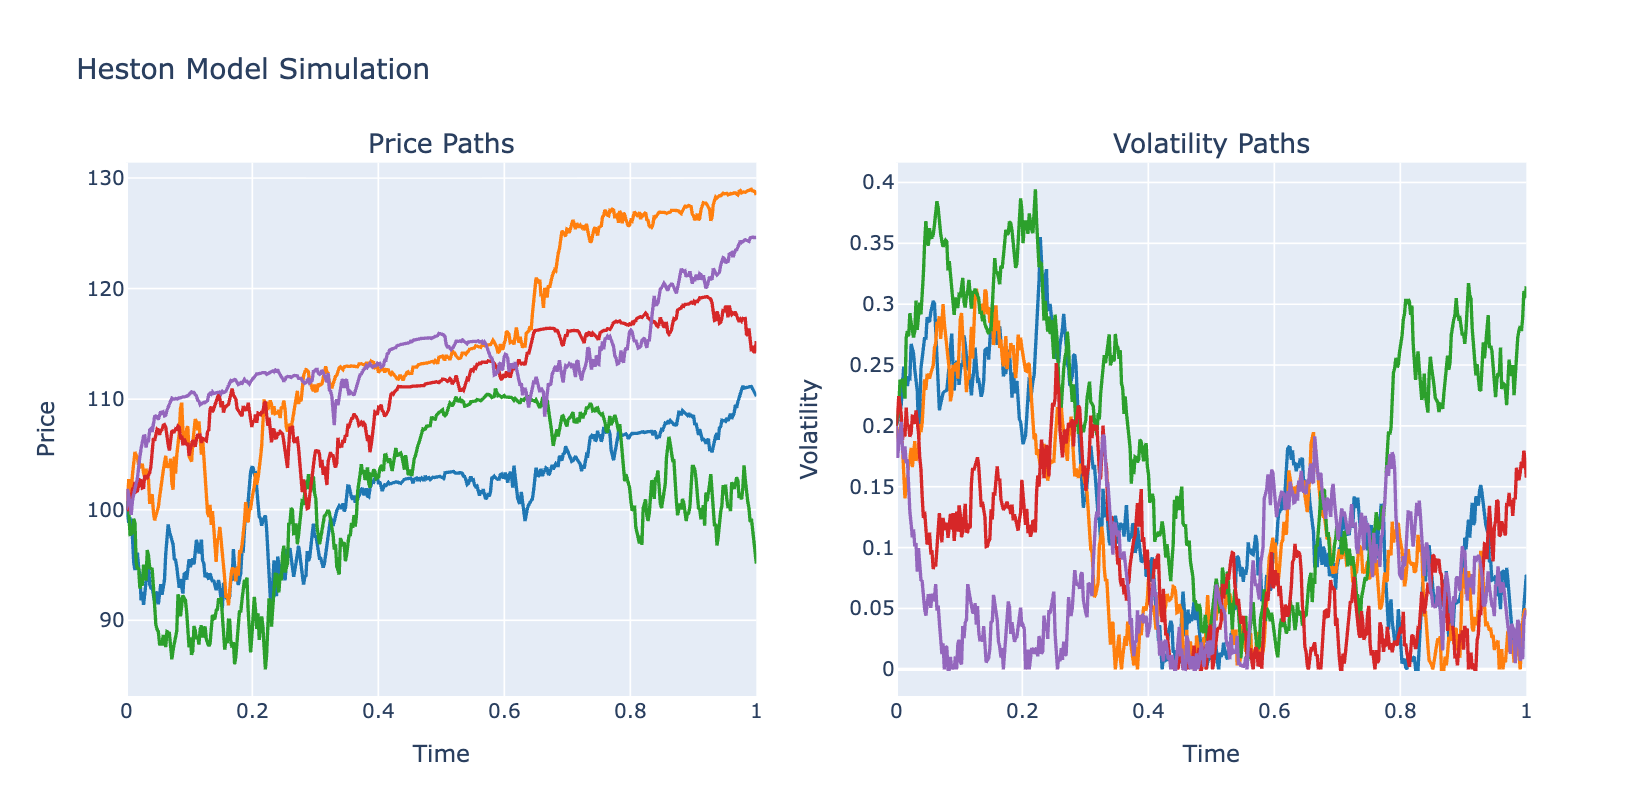
\includegraphics[width=\textwidth]{images/model_simulation.png}
  \caption{Simulated Heston model paths for the asset price and variance process using a Milstein-corrected Euler scheme ($S_0=100$, $v_0=0.04$, $\kappa=2.0$, $\theta=0.04$, $\sigma=0.6$, $\rho=-0.7$, $r=0.05$, $q=0.02$, $T=1$, $N=512$).}
  \label{fig:heston-simulation-app}
\end{figure}

\begin{figure}[H]
  \centering
  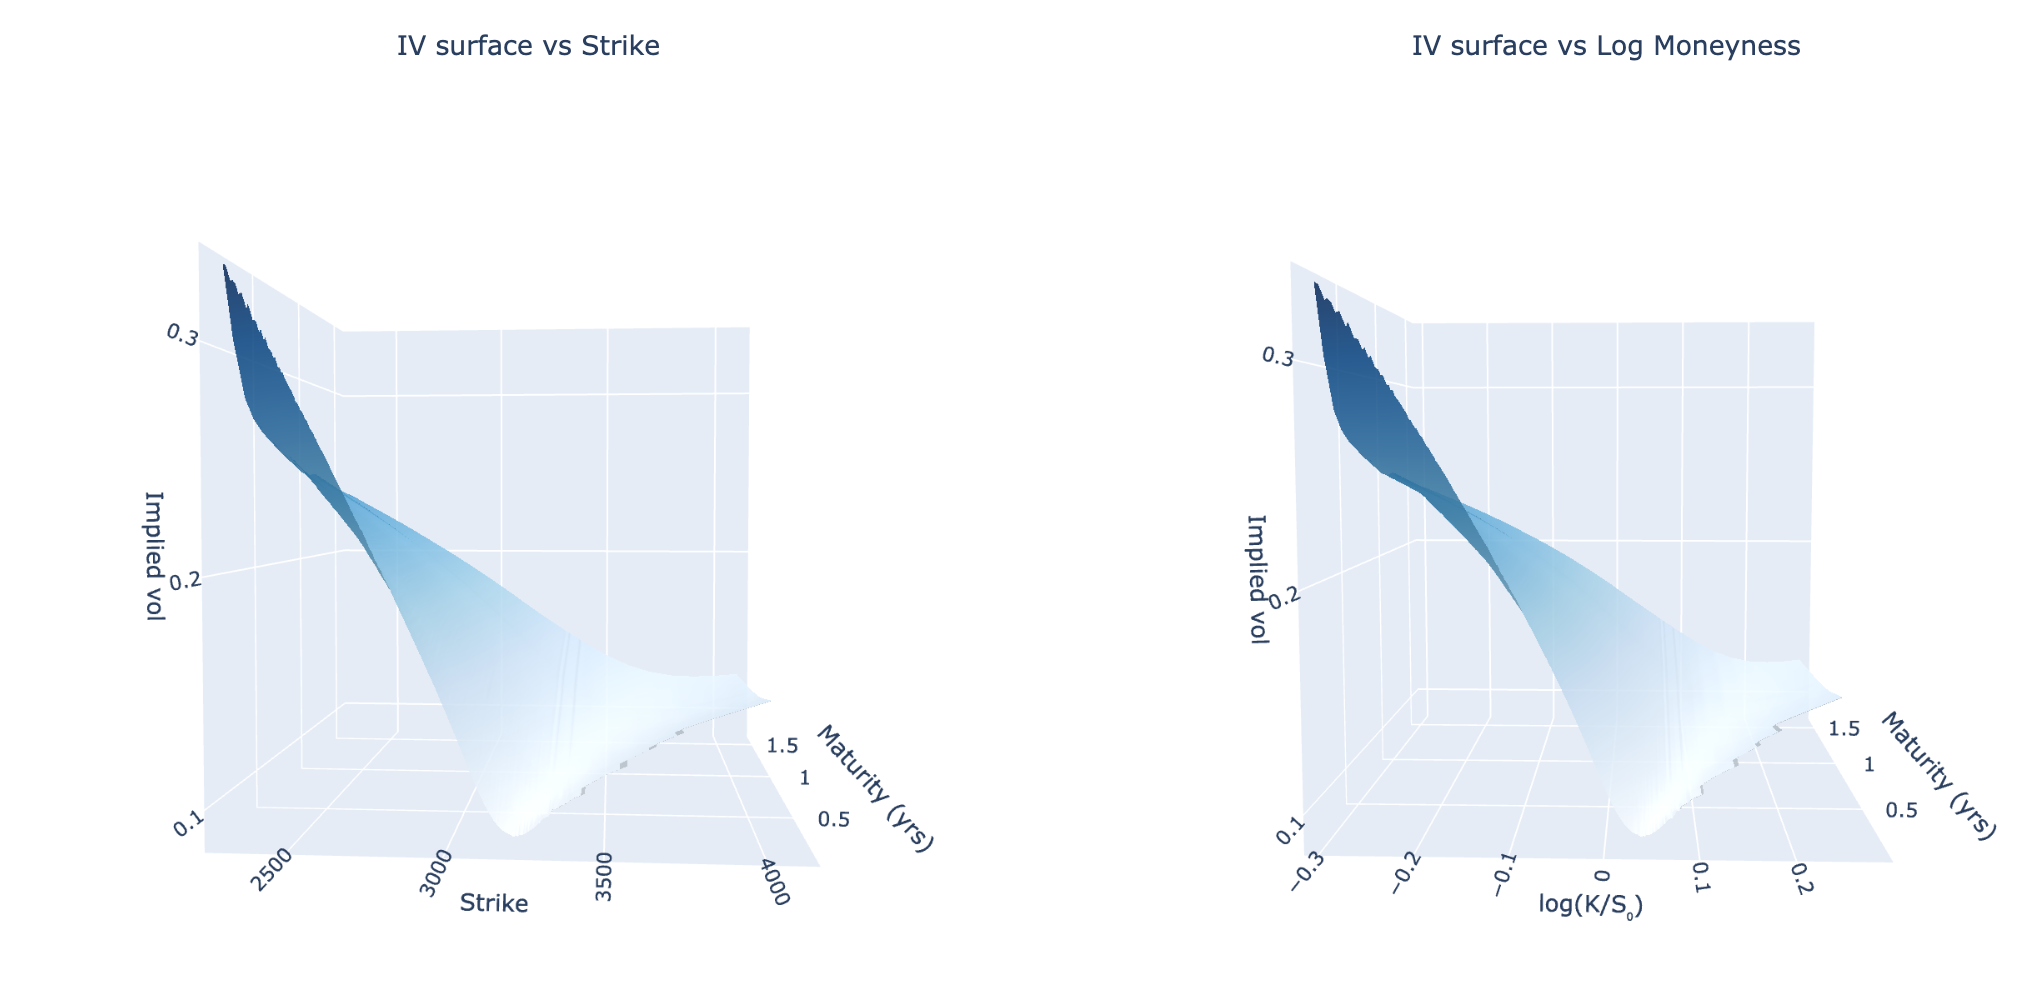
\includegraphics[width=\textwidth]{images/implied_vol_market_only.png}
  \caption{Market implied volatility surface from S\&P 500 options data (13 November 2019, $S_0 = 3094$) after data cleaning and arbitrage filtering, plotted against strike and log-moneyness.}
  \label{fig:market-iv-surface-app}
\end{figure}

\begin{figure}[H]
  \centering
  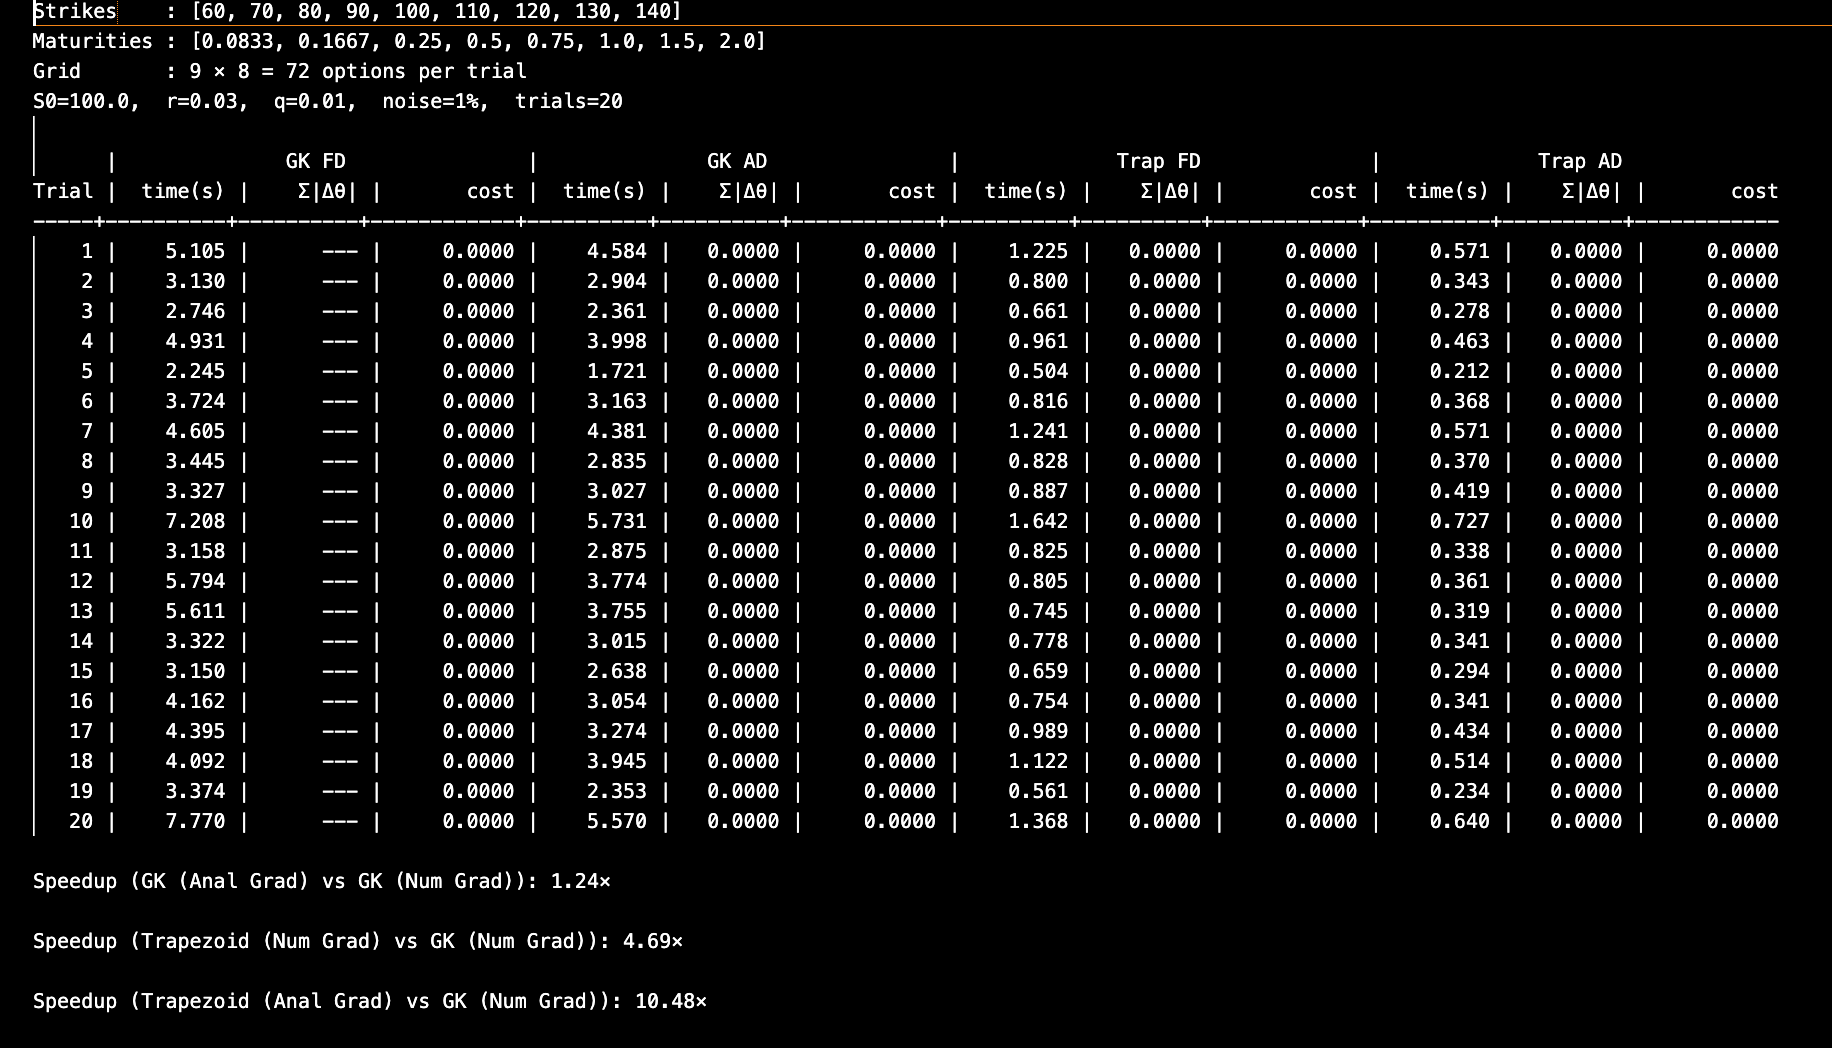
\includegraphics[width=\textwidth]{images/calibration_speed_experiment.png}
  \caption{Calibration speed experiment: wall time and $\sum|\Delta\sigma|$ relative to the GK baseline across 20 random Heston parameter draws satisfying the Feller condition.}
  \label{fig:calibration-speed-app}
\end{figure}

\begin{figure}[H]
  \centering
  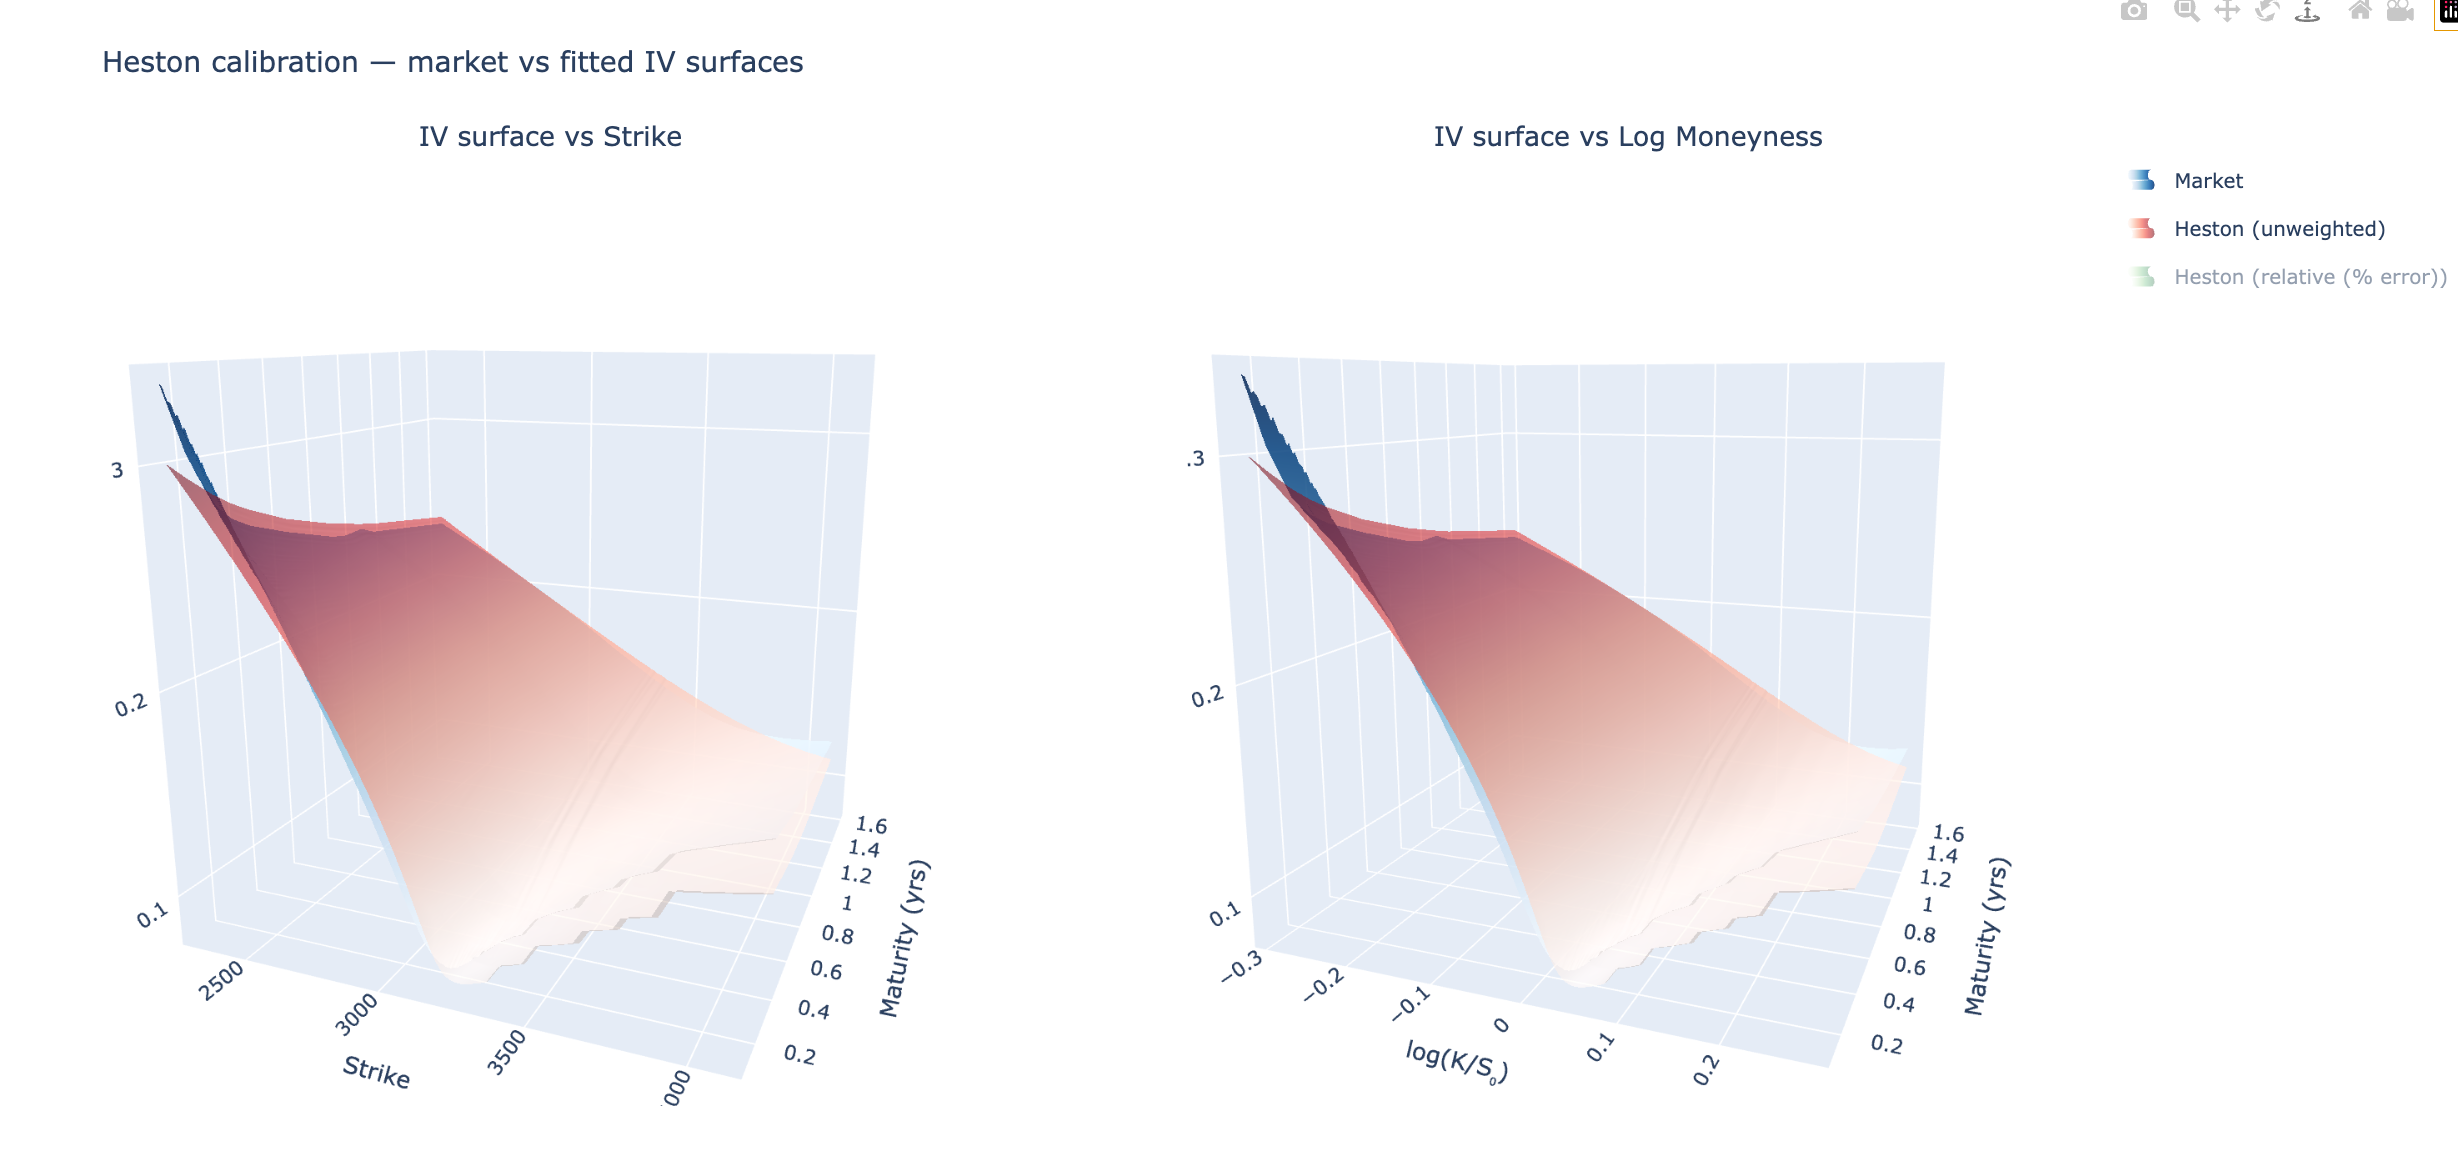
\includegraphics[width=\textwidth]{images/unweighted.png}
  \caption{Heston model fitted IV surface (unweighted calibration) vs.\ market implied volatility surface, S\&P 500 options (13 November 2019, $S_0 = 3094$).}
  \label{fig:iv-fit-unweighted-app}
\end{figure}

\begin{figure}[H]
  \centering
  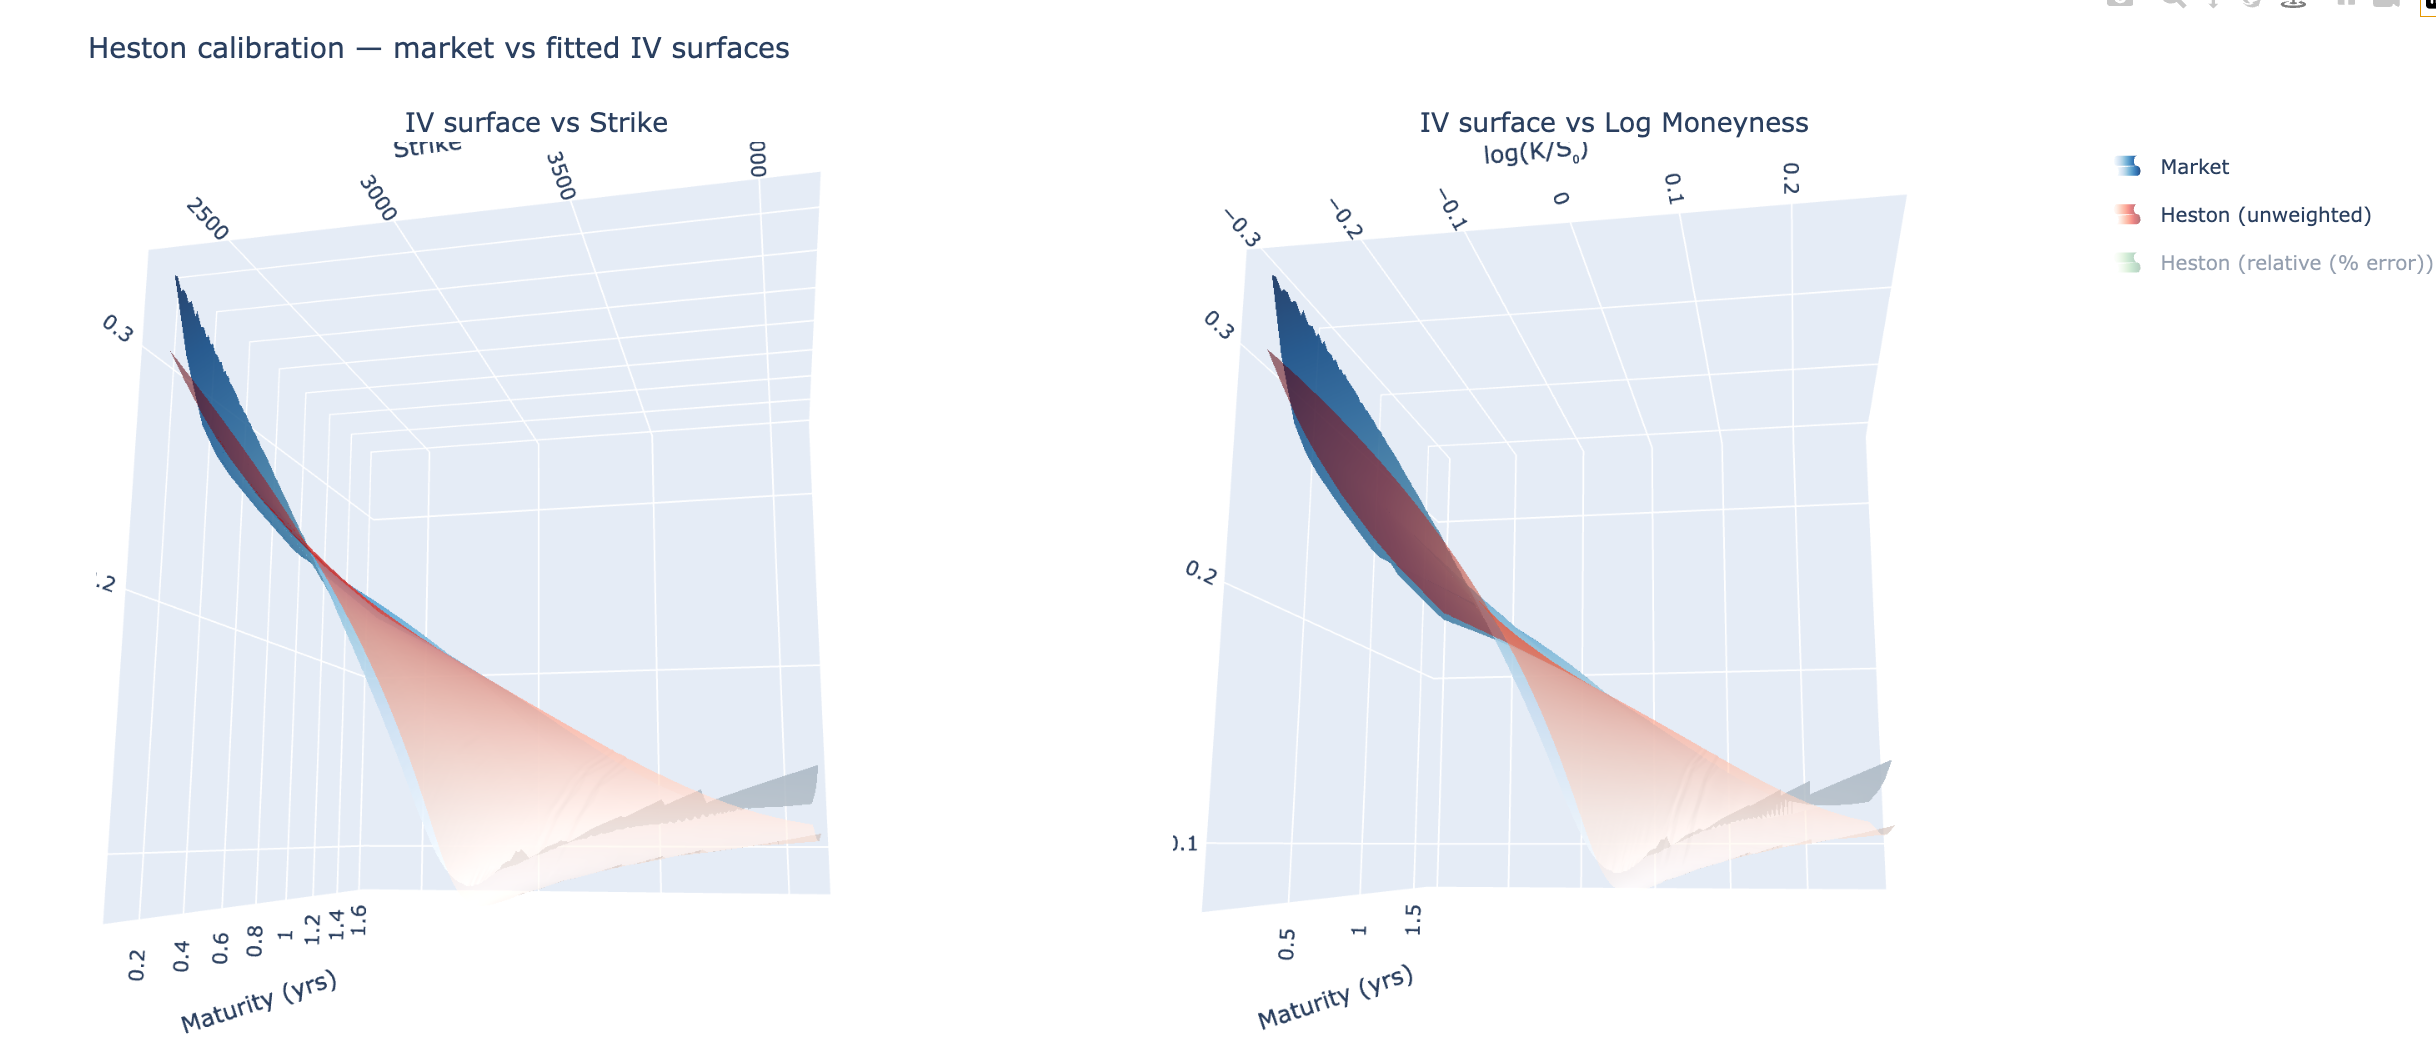
\includegraphics[width=\textwidth]{images/unweighted2.png}
  \caption{Alternative viewing angle of the Heston fitted IV surface (unweighted calibration) vs.\ market implied volatility surface, S\&P 500 options (13 November 2019, $S_0 = 3094$).}
  \label{fig:iv-fit-unweighted2}
\end{figure}

\begin{figure}[H]
  \centering
  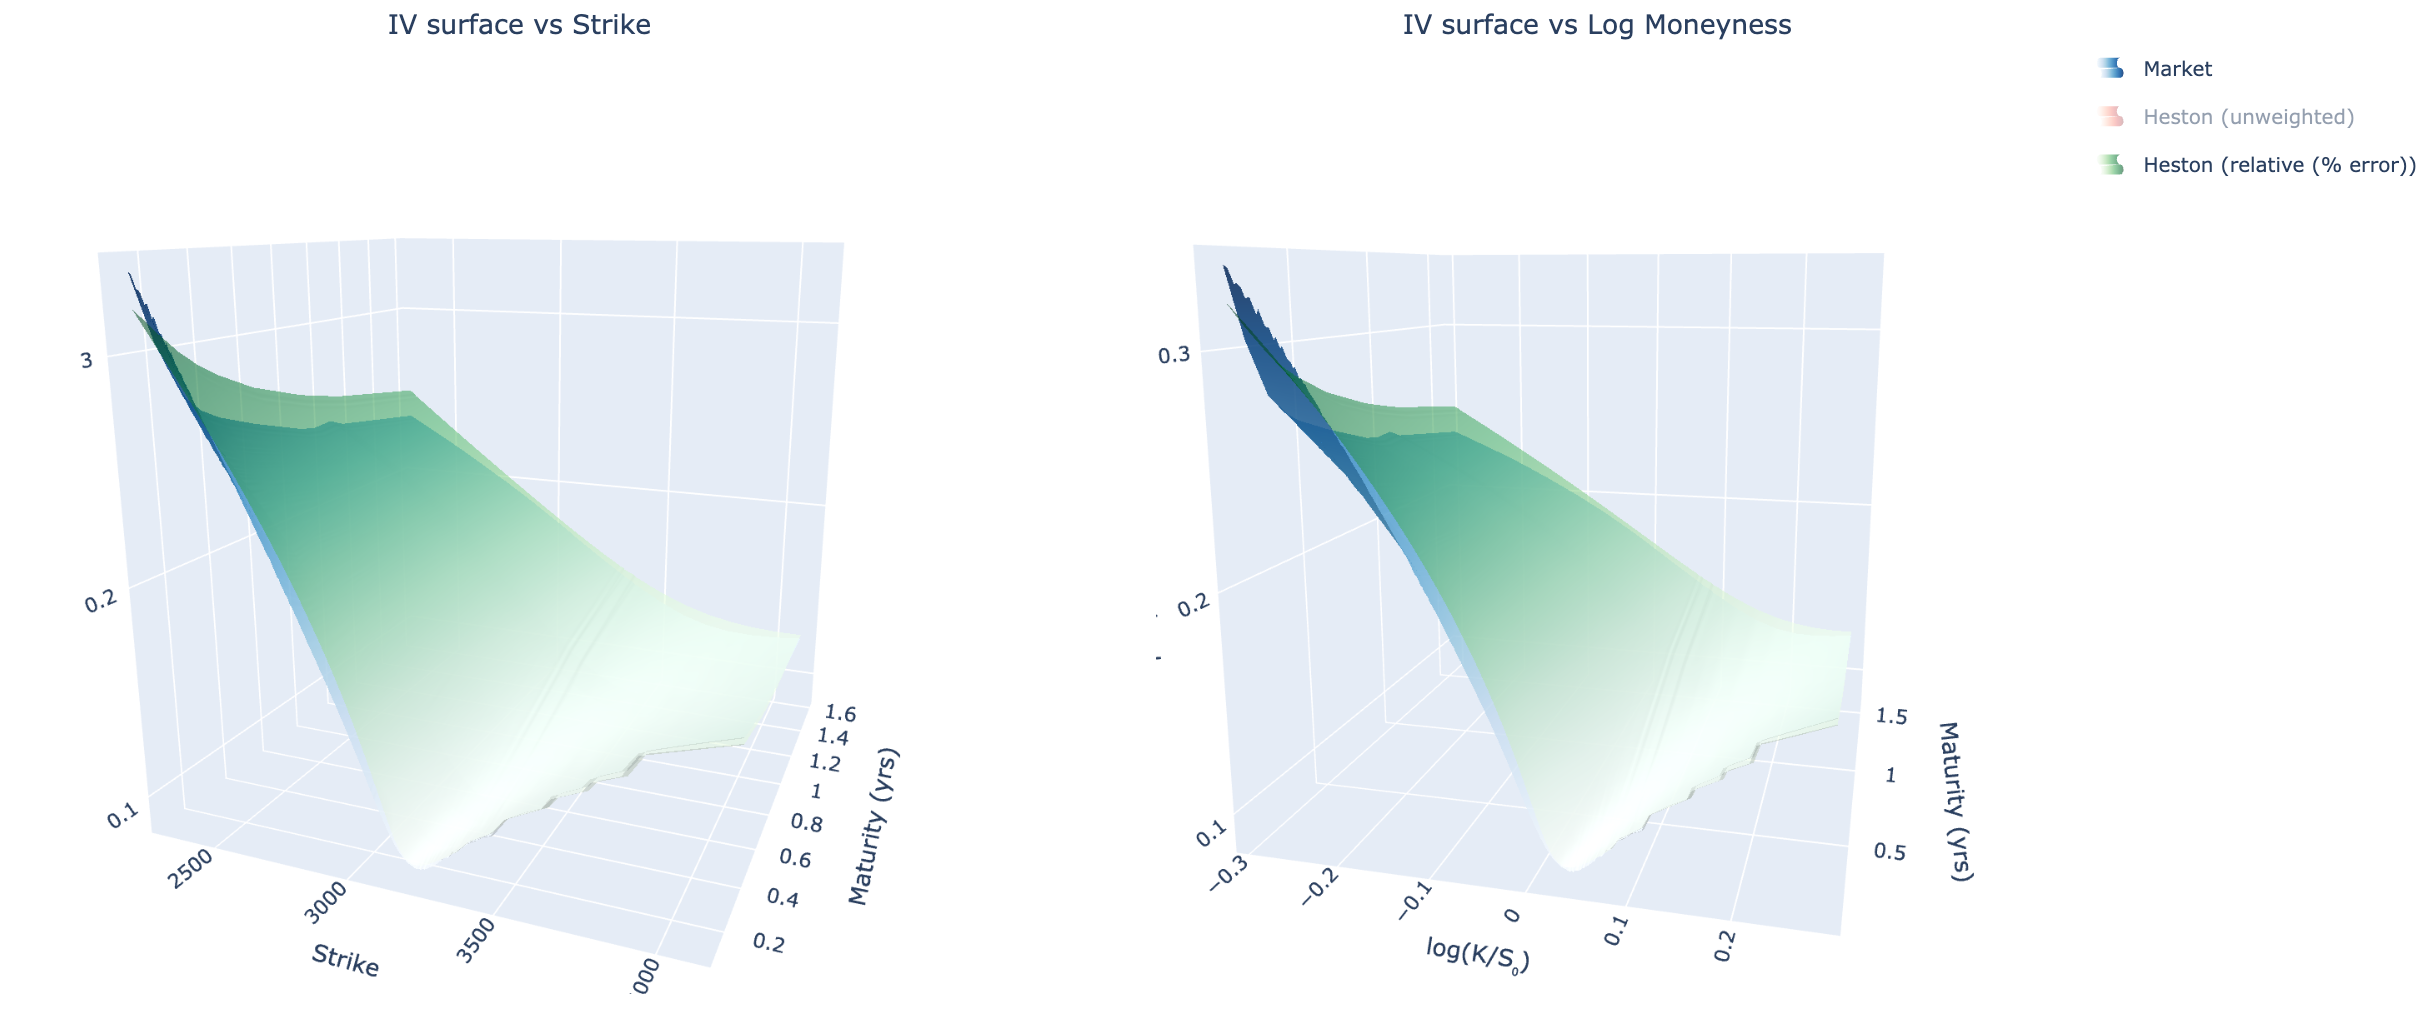
\includegraphics[width=\textwidth]{images/relative.png}
  \caption{Heston model fitted IV surface (relative error weighting) vs.\ market implied volatility surface, S\&P 500 options (13 November 2019, $S_0 = 3094$).}
  \label{fig:iv-fit-relative-app}
\end{figure}

\begin{figure}[H]
  \centering
  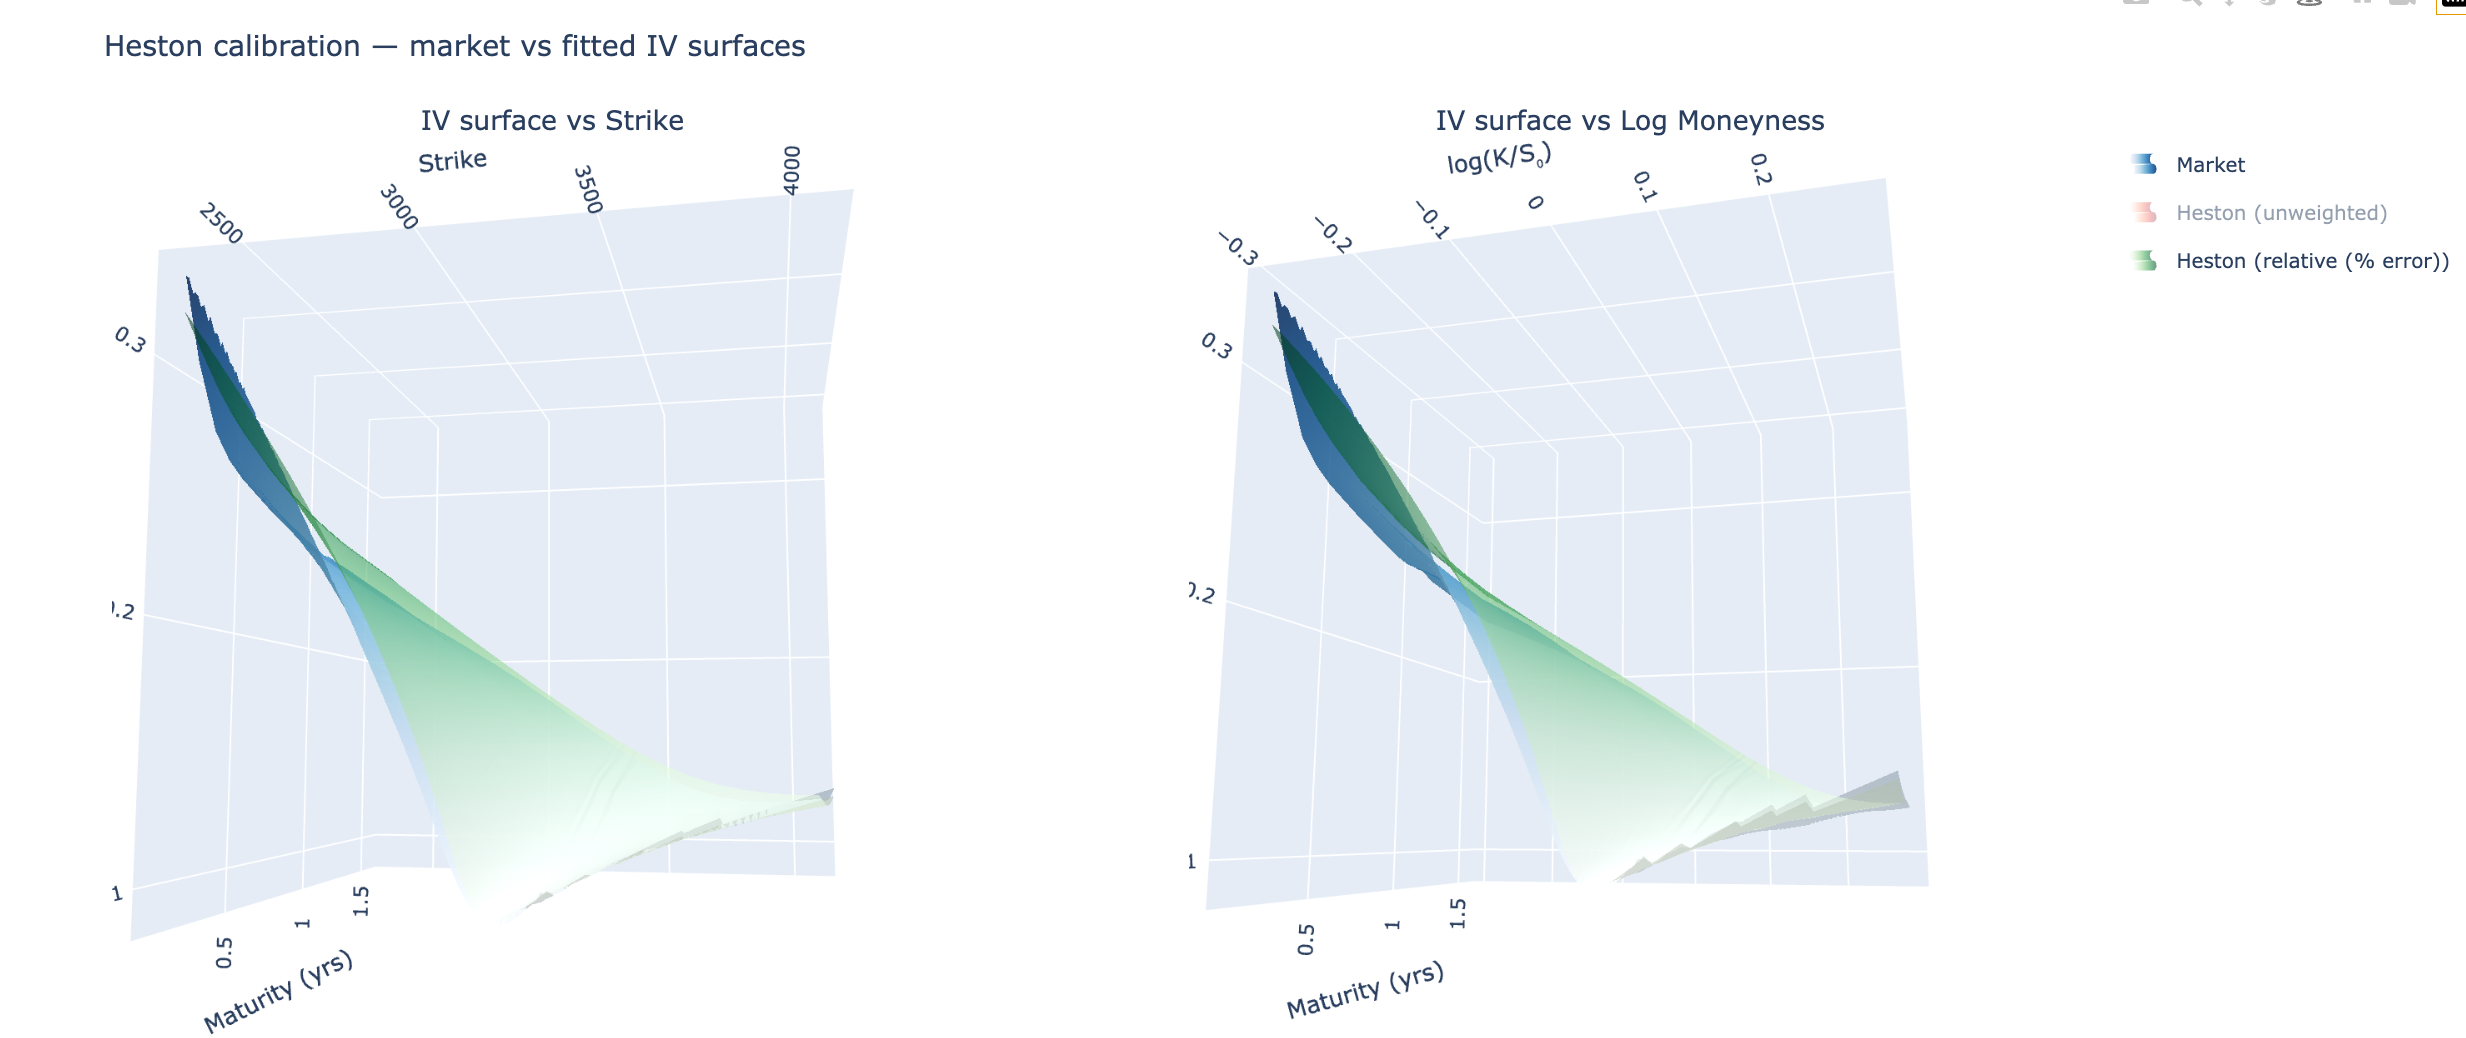
\includegraphics[width=\textwidth]{images/relative2.png}
  \caption{Alternative viewing angle of the Heston fitted IV surface (relative error weighting) vs.\ market implied volatility surface, S\&P 500 options (13 November 2019, $S_0 = 3094$).}
  \label{fig:iv-fit-relative2}
\end{figure}

\subsection{code}
The code generated making this project can be found in the github repo~\cite{github_repo}, in there is a read me explaining the
code structure, and how to run it replicating everything with seeding 
